\documentclass[11pt]{article}

\usepackage[margin=1in]{geometry}
\usepackage{amsmath,amssymb,amsthm}
\usepackage{bm}
\usepackage{booktabs}
\usepackage{graphicx}
\usepackage{tikz}
\usetikzlibrary{arrows.meta,positioning,calc,backgrounds,fit,shapes.geometric,shapes.misc}
\usepackage[colorlinks=true,linkcolor=blue,citecolor=blue,urlcolor=blue]{hyperref}

\newtheorem{proposition}{Proposition}
\newtheorem{corollary}{Corollary}
\newtheorem{remark}{Remark}

\newcommand{\Rup}{\mathcal{R}_{\mathrm{up}}}
\newcommand{\Rdown}{\mathcal{R}_{\mathrm{down}}}
\newcommand{\Rtot}{\mathcal{R}_{\mathrm{tot}}}
\newcommand{\kbr}{k_{\mathrm{br}}}
\newcommand{\qtum}{q_{\mathrm{tum}}}

\title{\vspace{-2em}Flow--Field Equivalence of a Bridged Vessel Break:\\
Schur--Complement Port Reduction and a Resistance--Fraction Tolerance}
\author{Methods note --- thermoembolization 1D transport model}
\date{\today}

\begin{document}
\maketitle
\vspace{-1.5em}

\begin{abstract}
\noindent
A segmentation-induced discontinuity in the extracted hepatic-artery centerline
severs the 1D Hagen--Poiseuille flow network of Amare et al.\ and produces
catastrophic false-negative predictions of bolus delivery. We formalize the
alternative in which flow is routed from the inflow terminal, through the 3D
tissue domain, and back into the outflow terminal. We show that, for any linear
port-to-port bridge, the entire 3D block collapses via a Schur complement to a
single effective conductance $\kbr$, and that the bridged network reproduces the
intact tumor flow \emph{exactly} iff $\kbr$ equals the conductance of the missing
segment. We then derive the tolerance around that exact condition: the fractional
error in delivered flow equals the fractional error in $\kbr$ scaled by
$\phi$, the fraction of the inlet-to-tumor path resistance contributed by the
broken segment. Because segment conductance scales as $R^4$, $\phi$ is small for
proximal/large-radius breaks and approaches unity for distal/small-radius breaks
near the tumor, giving a computable, per-break map of when a break can be safely
bridged and when accurate bridge calibration is required.
\end{abstract}

\section{Governing 1D flow model (Amare et al.)}
\label{sec:model}

We adopt the reduced blood-flow model of Amare et al.\ verbatim. The extracted
centerline is a graph in which each voxel is a pressure node and each connection a
Hagen--Poiseuille element. For the element joining nodes $i$ and $j$,
\begin{equation}
q_{ij} = k_{ij}\,(P_i - P_j),
\qquad
k_{ij} = \frac{\pi R_{ij}^{4}}{8\mu L_{ij}},
\label{eq:hp}
\end{equation}
where $R_{ij}$, $L_{ij}$ are the radius and length of the element and $\mu$ the
blood viscosity. Mass balance at every interior node $i$ reads
\begin{equation}
\sum_{j\in N_i} k_{ij}\,(P_i - P_j) = 0,
\label{eq:mass}
\end{equation}
a Dirichlet inlet condition fixes the root pressure,
\begin{equation}
P_{\mathrm{root}} = P_{\mathrm{MAP}},
\label{eq:dirichlet}
\end{equation}
and each terminal node carries a Neumann/sink condition coupling it to the
unsegmented bed at central venous pressure through a lumped conductance
$\gamma_a/\mu$,
\begin{equation}
\sum_{j\in N_i} k_{ij}\,(P_i - P_j) \;+\; \frac{\gamma_a}{\mu}\,(P_{\mathrm{CVP}} - P_i) = 0.
\label{eq:neumann}
\end{equation}
Assembling \eqref{eq:hp}--\eqref{eq:neumann} over all nodes gives the linear system
\begin{equation}
L\,\bm{P} = \bm{f},
\label{eq:linsys}
\end{equation}
where $L$ is a weighted graph Laplacian (symmetric positive definite once the
Dirichlet condition is imposed) with off-diagonal entries $-k_{ij}$, and $\bm{f}$
encodes the boundary data. All quantities of interest---in particular the flow
delivered toward a tumor bed---are linear functionals of the solution $\bm{P}$ of
\eqref{eq:linsys}. This linearity is the sole structural fact the results below
require.

\section{The break and its 3D bridge}
\label{sec:bridge}

Let a single element between an \emph{inflow} node $a$ and an \emph{outflow} node
$b$ be lost to a segmentation break. In the intact network the two nodes are joined
by the Hagen--Poiseuille conductance
\begin{equation}
k_{ab} = \frac{\pi R_{ab}^{4}}{8\mu L_{ab}},
\label{eq:kab}
\end{equation}
and the subtree feeding the tumor hangs off $b$. We denote by $\qtum$ the total flow
crossing $b$ toward that subtree.

When the element is removed, we reconnect $a$ and $b$ through the 3D domain: the
inflow terminal acts as a source into a porous/Darcy tissue block and the outflow
terminal as a sink drawing from it. Provided the 3D transport is \emph{linear}
(Darcy, Stokes, or a further Hagen--Poiseuille sub-network---valid before
embolization-driven viscosity feedback sets in; see Remark~\ref{rem:nonlinear}),
the 3D block is a linear two-port probed only at $a$ and $b$.

\begin{figure}[t]
\centering
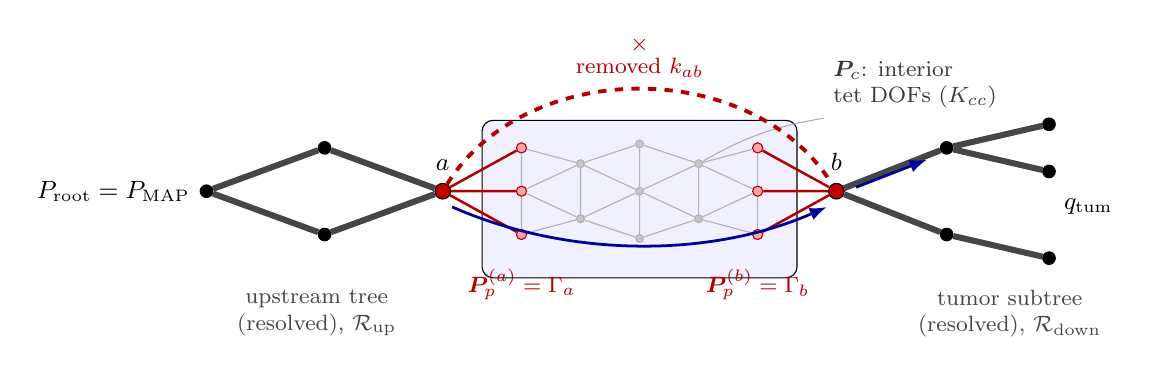
\begin{tikzpicture}[
  >={Latex[length=2.2mm]},
  node distance=6mm,
  vnode/.style={circle,draw,fill=black,inner sep=1.6pt},
  port/.style={circle,draw,fill=red!75!black,inner sep=2.0pt},
  pnode/.style={circle,draw=red!70!black,fill=red!35,inner sep=1.3pt},
  inode/.style={circle,draw=gray!60,fill=gray!45,inner sep=1.0pt},
  vessel/.style={line width=2.2pt,gray!55!black},
  tet/.style={gray!60,line width=0.4pt},
  flow/.style={->,line width=1.0pt,blue!60!black},
  lbl/.style={font=\small},
  slbl/.style={font=\footnotesize}
]

% ---- upstream tree (root -> a) ----
\node[vnode,label=left:{\small $P_{\mathrm{root}}=P_{\mathrm{MAP}}$}] (root) at (0,0) {};
\node[vnode] (u1) at (1.5,0.55) {};
\node[vnode] (u2) at (1.5,-0.55) {};
\draw[vessel] (root)--(u1);
\draw[vessel] (root)--(u2);
\node[port,label={[yshift=1pt]above:{\small $a$}}] (a) at (3.0,0) {};
\draw[vessel] (u1)--(a);
\draw[vessel] (u2)--(a);
\node[slbl,gray!55!black,align=center] at (1.4,-1.55) {upstream tree\\ (resolved), $\Rup$};

% ---- 3D bridge block: tet-mesh interior + two interface faces ----
\begin{scope}[on background layer]
\node[draw,rounded corners,fill=blue!6,minimum width=4.0cm,minimum height=2.0cm]
   (block) at (5.5,-0.1) {};
\end{scope}

% interface face Gamma_a (near a): a small column of interface DOFs (P_p)
\node[pnode] (pa1) at (4.0,0.55) {};
\node[pnode] (pa2) at (4.0,0.0) {};
\node[pnode] (pa3) at (4.0,-0.55) {};
% interface face Gamma_b (near b): interface DOFs (P_p)
\node[pnode] (pb1) at (7.0,0.55) {};
\node[pnode] (pb2) at (7.0,0.0) {};
\node[pnode] (pb3) at (7.0,-0.55) {};

% interior tet-mesh nodes (P_c)
\node[inode] (i1) at (4.75,0.35) {};
\node[inode] (i2) at (4.75,-0.35) {};
\node[inode] (i3) at (5.5,0.6) {};
\node[inode] (i4) at (5.5,0.0) {};
\node[inode] (i5) at (5.5,-0.6) {};
\node[inode] (i6) at (6.25,0.35) {};
\node[inode] (i7) at (6.25,-0.35) {};

% tetrahedral connectivity (K_cc among interior; K_pc to interface)
\draw[tet] (pa1)--(i1) (pa2)--(i1) (pa2)--(i2) (pa3)--(i2)
           (i1)--(i2) (i1)--(i3) (i1)--(i4) (i2)--(i4) (i2)--(i5)
           (i3)--(i4) (i4)--(i5) (i3)--(i6) (i4)--(i6) (i4)--(i7)
           (i5)--(i7) (i6)--(i7)
           (i6)--(pb1) (i6)--(pb2) (i7)--(pb2) (i7)--(pb3)
           (pa1)--(pa2) (pa2)--(pa3) (pb1)--(pb2) (pb2)--(pb3);

% lumped-port coupling: vessel port a -> interface face Gamma_a; Gamma_b -> port b
\draw[red!70!black,line width=0.9pt] (a)--(pa1) (a)--(pa2) (a)--(pa3);
\node[port,label={[yshift=1pt]above:{\small $b$}}] (b) at (8.0,0) {};
\draw[red!70!black,line width=0.9pt] (pb1)--(b) (pb2)--(b) (pb3)--(b);

% braces / labels for P_p and P_c
\node[slbl,red!70!black] at (4.0,-1.18) {$\bm{P}_p^{(a)}=\Gamma_a$};
\node[slbl,red!70!black] at (7.0,-1.18) {$\bm{P}_p^{(b)}=\Gamma_b$};
\node[slbl,gray!45!black,align=left] (pclbl) at (9.0,1.35) {$\bm{P}_c$: interior\\ tet DOFs ($K_{cc}$)};
\draw[gray!60,line width=0.4pt] (pclbl.south west) to[bend right=10] (i6);

% ---- removed direct a-b element ----
\draw[line width=1.4pt,red!70!black,dashed] (a) to[bend left=58] node[midway,above,slbl,red!70!black]{removed $k_{ab}$} (b);
\node[red!70!black] at ($(a)!0.5!(b)+(0,1.86)$) {\footnotesize $\times$};

% ---- flow route through the block ----
\draw[flow] ($(a)+(0.12,-0.20)$) .. controls (4.6,-0.85) and (6.4,-0.85) .. ($(b)+(-0.12,-0.20)$);

% ---- downstream tumor subtree (b -> tumor) ----
\node[vnode] (d1) at (9.4,0.55) {};
\node[vnode] (d2) at (9.4,-0.55) {};
\draw[vessel] (b)--(d1);
\draw[vessel] (b)--(d2);
\node[vnode] (t1) at (10.7,0.85) {};
\node[vnode] (t2) at (10.7,0.25) {};
\node[vnode] (t3) at (10.7,-0.85) {};
\draw[vessel] (d1)--(t1) (d1)--(t2) (d2)--(t3);
\draw[flow] (b)++(0.25,0.05) -- ++(0.9,0.35);
\node[slbl,gray!55!black,align=center] at (10.2,-1.55) {tumor subtree\\ (resolved), $\Rdown$};
\node[lbl,align=center] at (11.2,-0.2) {$\qtum$};

\end{tikzpicture}
\caption{Break geometry underlying the block system~\eqref{eq:blockbridge}. The
direct Hagen--Poiseuille element of conductance $k_{ab}$ (dashed, crossed) is lost to
the segmentation break. The 3D bridge is a tetrahedral mesh: its interior vertex DOFs
$\bm{P}_c$ (grey, coupled by $K_{cc}$) and its two \emph{interface} DOF sets
$\bm{P}_p=(\bm{P}_p^{(a)},\bm{P}_p^{(b)})$ on the coupling faces $\Gamma_a,\Gamma_b$
(red)---generally many nodes per face, not one. The 1D vessel connects to each face
as a single lumped port $a$ or $b$ (red edges), so recovering the two-DOF port vector
of \S\ref{sec:bridge} requires, in addition to eliminating $\bm{P}_c$
(Eq.~\eqref{eq:schur}), an interface-lumping constraint reducing each $\Gamma$ to one
pressure (Remark~\ref{rem:interface}). Flow enters at $a$, traverses the mesh, and
returns at $b$ to the resolved tumor subtree carrying $\qtum$; the resolved upstream
and downstream trees contribute $\Rup$ and $\Rdown$ of \S\ref{sec:tolerance}.}
\label{fig:break}
\end{figure}

\subsection{Schur-complement reduction of the 3D block}

Partition the degrees of freedom of the 3D bridge (Figure~\ref{fig:break}) into the
\emph{port} DOFs $\bm{P}_p$ and the \emph{interior} DOFs $\bm{P}_c$. For a
tetrahedral discretization the interior set $\bm{P}_c$ is the (large) collection of
mesh-vertex pressures coupled by the internal stiffness $K_{cc}$, while the port set
$\bm{P}_p=(\bm{P}_p^{(a)},\bm{P}_p^{(b)})$ collects the interface vertices on the two
coupling faces $\Gamma_a,\Gamma_b$ where the 1D vessel meets the tissue---in general
$|\bm{P}_p|=|\Gamma_a|+|\Gamma_b|\gg 2$, not a single node per port
(see Remark~\ref{rem:interface}). The discrete linear operator (Darcy stiffness /
internal Laplacian) has the block form
\begin{equation}
\begin{pmatrix} K_{pp} & K_{pc} \\ K_{cp} & K_{cc} \end{pmatrix}
\begin{pmatrix} \bm{P}_p \\ \bm{P}_c \end{pmatrix}
=
\begin{pmatrix} \bm{g}_p \\ \bm{0} \end{pmatrix},
\label{eq:blockbridge}
\end{equation}
where the interior right-hand side is zero because sources enter only at the ports.
Eliminating the interior unknowns, $\bm{P}_c = -K_{cc}^{-1}K_{cp}\bm{P}_p$, yields
the \emph{Schur complement} of $K_{cc}$,
\begin{equation}
S \;=\; K_{pp} - K_{pc}\,K_{cc}^{-1}\,K_{cp}
\;\in\;\mathbb{R}^{|\bm{P}_p|\times|\bm{P}_p|},
\qquad
S\,\bm{P}_p = \bm{g}_p,
\label{eq:schur}
\end{equation}
a dense face-to-face conductance matrix over all interface DOFs. The 1D network
resolves each face only as a single lumped pressure and net flux, so we impose an
interface-lumping constraint---$\bm{P}_p^{(a)}\!\equiv\!P_a\bm{1}$,
$\bm{P}_p^{(b)}\!\equiv\!P_b\bm{1}$ (equal pressure across each face, with the face
flux as its conjugate; Remark~\ref{rem:interface})---which reduces $S$ to the
$2\times2$ port operator $\hat S$. For a two-port with no internal sources $\hat S$
has the conductance (weighted-Laplacian) structure
\begin{equation}
\hat S =
\begin{pmatrix} \kbr & -\kbr \\ -\kbr & \kbr \end{pmatrix},
\qquad
\kbr \;\equiv\; \bigl(\hat S\bigr)_{aa} = -\bigl(\hat S\bigr)_{ab} \;>\;0,
\label{eq:kbr}
\end{equation}
so that the port relation collapses to a single scalar,
\begin{equation}
\boxed{\;q_{a\to b}^{\mathrm{bridge}} = \kbr\,(P_a - P_b).\;}
\label{eq:portlaw}
\end{equation}

\begin{remark}[What $\bm{P}_p$ is, and why lumping is a modeling choice]
\label{rem:interface}
The port set $\bm{P}_p$ is \emph{not} two scalars in a tetrahedral bridge: it is the
set of interface vertices on the coupling faces $\Gamma_a,\Gamma_b$, and the
interior elimination \eqref{eq:schur} produces a dense $|\bm{P}_p|\times|\bm{P}_p|$
face-to-face conductance, not the $2\times2$ of \eqref{eq:kbr}. The single scalar
$\kbr$ emerges only after a \emph{second} reduction that lumps each face to one DOF.
The lumping rule---uniform face pressure, flux-weighted average, or a single-node
coupling---is a modeling choice that changes $\kbr$, exactly the identifiability
question already present in the terminal $\gamma_a$ closure of \eqref{eq:neumann},
now posed at an interior interface. All results below hold once a lumping is fixed;
the sensitivity of $\kbr$ to that choice is itself worth reporting.
\end{remark}

\begin{proposition}[Complete port characterization]
\label{prop:port}
However complex the internal geometry, permeability field, or discretization of the
3D bridge, its effect on the surrounding 1D network is fully described by the single
effective conductance $\kbr$ of \eqref{eq:kbr}. All of gap length, gap width, tissue
permeability, and bridge topology enter the global flow solve \emph{only} through
$\kbr$.
\end{proposition}

\noindent
Consequently the bridged network is identical to a network in which $a$ and $b$ are
joined by one Hagen--Poiseuille-like element of conductance $\kbr$. The break has
been reduced to a single edge weight.

\section{Exact flow equivalence}
\label{sec:exact}

Compare two networks that are identical everywhere---same upstream tree, same
downstream tumor subtree, same terminal $\gamma_a$ couplings---except for the single
edge between $a$ and $b$: the intact network carries weight $k_{ab}$
\eqref{eq:kab}, the bridged network carries weight $\kbr$ \eqref{eq:kbr}.

\begin{proposition}[Exact equivalence]
\label{prop:exact}
Let $\qtum(k)$ denote the tumor-directed flow when the $a$--$b$ edge has conductance
$k$, all else fixed. Then $\qtum$ is a rational (M\"obius) function of $k$, and
\begin{equation}
\qtum^{\mathrm{broken}} = \qtum^{\mathrm{intact}}
\quad\Longleftrightarrow\quad
\kbr = k_{ab} = \frac{\pi R_{ab}^{4}}{8\mu L_{ab}}.
\label{eq:exact}
\end{equation}
\end{proposition}

\begin{proof}
Changing a single edge weight is a rank-one modification of the Laplacian in
\eqref{eq:linsys}: $L(k) = L_0 + k\,\bm{e}_{ab}\bm{e}_{ab}^{\!\top}$, where
$\bm{e}_{ab} = \bm{u}_a - \bm{u}_b$ is the incidence vector of the edge. By the
Sherman--Morrison formula the solution $\bm{P}(k) = L(k)^{-1}\bm{f}$ is a
componentwise M\"obius function of $k$, hence so is any linear functional
$\qtum(k)$. A M\"obius function is injective on the physical branch $k>0$
(its derivative does not vanish), so $\qtum(k_1)=\qtum(k_2)$ with $k_1,k_2>0$
forces $k_1=k_2$. Taking $k_1=\kbr$, $k_2=k_{ab}$ gives \eqref{eq:exact}.
\end{proof}

\begin{remark}[Calibration target: unresolved lumen, not bulk tissue]
\label{rem:lumen}
Equation~\eqref{eq:exact} states the bridging requirement precisely: the 3D bridge
must reproduce the conductance of the \emph{vessel segment it replaced}. A break is
almost always unresolved lumen rather than parenchyma, so $k_{ab}$ is a
high-conductance channel. Bridging instead with bulk-tissue permeability gives
$\kbr \ll k_{ab}$, starving the downstream tumor and reintroducing the
false-negative. The correct bridge is therefore a vessel-like channel whose
port-reduced conductance matches $k_{ab}$---the interior analogue of the terminal
$\gamma_a$ closure in \eqref{eq:neumann}, now applied to an \emph{interior} gap.
\end{remark}

\section{Tolerance: the resistance-fraction \texorpdfstring{$\phi$}{phi}}
\label{sec:tolerance}

Exact equality requires the true $k_{ab}$, which is unknown precisely where the
vessel broke. The operational question is therefore how far $\kbr$ may deviate from
$k_{ab}$ before the tumor flow changes appreciably. Reduce the inlet-to-tumor path
to three conductances in series: the port-reduced upstream resistance $\Rup$ seen
at $a$, the broken segment $1/k$, and the port-reduced downstream resistance
$\Rdown$ seen from $b$ into the tumor bed. The delivered flow is
\begin{equation}
\qtum(k) = \frac{\Delta P}{\Rtot(k)},
\qquad
\Rtot(k) = \Rup + \frac{1}{k} + \Rdown,
\label{eq:series}
\end{equation}
with $\Delta P$ the effective driving pressure across the path. Define the
\emph{resistance fraction} of the broken segment in the intact network,
\begin{equation}
\boxed{\;
\phi \;=\; \frac{1/k_{ab}}{\Rtot(k_{ab})}
\;=\; \frac{1/k_{ab}}{\Rup + 1/k_{ab} + \Rdown}
\;\in (0,1).
\;}
\label{eq:phi}
\end{equation}

\noindent
Two points on this definition. First, $\phi$ is built from the \emph{true} segment
conductance $k_{ab}$ and the \emph{intact} total resistance $\Rtot(k_{ab})$---not
from the bridge $\kbr$---because $\phi$ is a property of the anatomy being
reproduced, the fixed reference against which any bridge error is judged. It answers
``how much leverage does this location have over the delivered flow?'' and that
leverage is a fact about the vessel that should be true, evaluated as if the segment
were still present, independent of whatever bridge one later inserts. Using $\kbr$
here would make $\phi$ move every time the bridge changed and would forfeit exactly
the property that makes it useful: computability from the resolved network
\emph{before} any bridge value is chosen (Corollary~\ref{cor:map}).
Second, the two conductances play distinct roles that the tolerance
result~\eqref{eq:tol} keeps separate. $k_{ab}$ sets the \emph{reference}---where the
flow should land---and enters only through $\phi$, the sensitivity; $\kbr$ is the
\emph{controllable variable}, and enters only through its relative deviation
$\delta=(\kbr-k_{ab})/k_{ab}$. The product $\phi\,\delta$ then factors cleanly into
``how sensitive is the flow to a bridge error here'' ($\phi$, from $k_{ab}$) times
``how large is my bridge error'' ($\delta$, from $\kbr$). Formally, $\phi$ is the
sensitivity $\partial q_{\mathrm{tum}}/\partial(1/k)$ evaluated at the
exact-equivalence operating point $k=k_{ab}$ of Proposition~\ref{prop:exact}, since a
first-order tolerance is a statement about deviations \emph{away from} the correct
value---and the correct value is $k_{ab}$.

\begin{proposition}[First-order flow tolerance]
\label{prop:tol}
Let the bridge conductance carry a relative error $\delta = (\kbr - k_{ab})/k_{ab}$.
Then to first order the relative error in delivered tumor flow is
\begin{equation}
\frac{\qtum^{\mathrm{broken}} - \qtum^{\mathrm{intact}}}{\qtum^{\mathrm{intact}}}
\;\approx\; \phi\,\frac{\delta}{1+\delta}
\;\approx\; \phi\,\delta
\qquad (|\delta|\ll 1).
\label{eq:tol}
\end{equation}
\end{proposition}

\begin{proof}
From \eqref{eq:series}, $\qtum \propto \Rtot^{-1}$. Perturbing $k\!:\,k_{ab}\to\kbr$
changes only the middle term, $1/k_{ab}\to 1/\kbr = (1/k_{ab})/(1+\delta)$, so
\[
\Rtot(\kbr) = \Rtot(k_{ab}) - \frac{1}{k_{ab}}\frac{\delta}{1+\delta}.
\]
Dividing by $\Rtot(k_{ab})$ and using \eqref{eq:phi},
$\Rtot(\kbr)/\Rtot(k_{ab}) = 1 - \phi\,\delta/(1+\delta)$, and since
$\qtum^{\mathrm{broken}}/\qtum^{\mathrm{intact}} = \Rtot(k_{ab})/\Rtot(\kbr)$,
inverting and linearizing gives \eqref{eq:tol}.
\end{proof}

\noindent
The interpretation is the operational payoff. The delivered-flow error is the
bridge-conductance error \emph{attenuated by} $\phi$:
\begin{itemize}
\item \textbf{$\phi \ll 1$ (wide tolerance).} When the broken segment contributes
little of the path resistance, even a large mis-estimate of $\kbr$ barely moves the
tumor flow. Because $1/k_{ab}\propto L_{ab}/R_{ab}^4$, this is the regime of
\emph{proximal, large-radius} breaks: the path resistance is dominated by the small
distal vessels downstream, which the break leaves untouched. Here a break may be
bridged crudely---or even left as any reasonable high-conductance channel---without
harming the delivered-dose prediction.
\item \textbf{$\phi \to 1$ (narrow tolerance).} When the broken segment is itself
the dominant resistance---\emph{distal, small-radius} breaks near the tumor, where
$R_{ab}^4$ is smallest---the tumor flow tracks $\kbr$ almost one-for-one and the
bridge must be calibrated accurately to $k_{ab}$.
\end{itemize}

\begin{corollary}[Per-break tolerance map, computable without the gap]
\label{cor:map}
$\Rup$ and $\Rdown$ are Schur-reduced resistances of the \emph{resolved} network
at $a$ and $b$ and are obtained from the intact solve; $k_{ab}$ enters $\phi$ only
through the assumed gap geometry. Hence $\phi$ can be estimated for every candidate
break from the surrounding resolved vasculature, yielding an a priori map of which
breaks fall in the wide- versus narrow-tolerance regime before any bridging is
performed.
\end{corollary}

\section{Worked example: proximal versus distal break}
\label{sec:example}

To make the tolerance concrete we take a single three-generation path from the
injection site to a tumor terminal (Remark~\ref{rem:generations}), with radii
tapering from a lobar artery to a subsegmental feeder and roughly constant segment
length. Radii and lengths, and the resulting Hagen--Poiseuille conductances
\eqref{eq:kab}, are listed in Table~\ref{tab:tree}, and the three break locations are
shown on the path in Figure~\ref{fig:tree}. The downstream tumor-bed
closure is set to $40\%$ and the proximal (aorta/celiac) feed to $5\%$ of the summed
segment resistance, so that---as in vivo---the small distal vessels plus bed carry
most of the path resistance.

\begin{table}[h]
\centering
\small
\begin{tabular}{lccccc}
\toprule
segment & $R$ (mm) & $L$ (mm) & $k_{ab}$ (SI) & $\phi$ & $\delta$ for $10\%$ flow error \\
\midrule
g1 (lobar, proximal)      & $1.20$ & $15$ & $1.55\times10^{-8}$ & $0.011$ & $\pm\,900\%$ \\
g2 (segmental)            & $0.70$ & $12$ & $2.25\times10^{-9}$ & $0.077$ & $\pm\,130\%$ \\
g3 (subsegmental, distal) & $0.40$ & $10$ & $2.87\times10^{-10}$ & $0.602$ & $\pm\,17\%$ \\
\bottomrule
\end{tabular}
\caption{Three-generation delivery path. A break in the proximal large-radius
segment (g1) contributes almost none of the path resistance ($\phi=0.011$) and so
tolerates an enormous bridge-conductance error; a break in the distal small-radius
feeder (g3) is itself the dominant resistance ($\phi=0.602$) and tolerates only a
narrow error band. The $81\times$ spread in $\phi$ tracks the
$(1.20/0.40)^4=81$ ratio of the fourth powers of the radii.}
\label{tab:tree}
\end{table}

\begin{figure}[h]
\centering
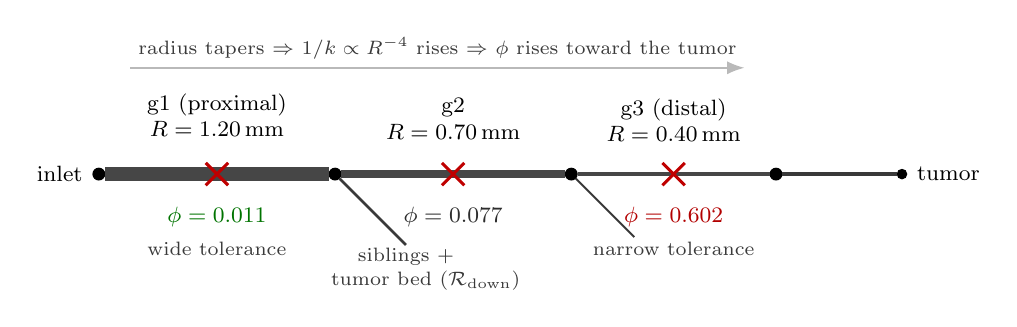
\begin{tikzpicture}[
  >={Latex[length=2.2mm]},
  vnode/.style={circle,draw,fill=black,inner sep=1.5pt},
  term/.style={circle,draw,fill=black,inner sep=1.2pt},
  brk/.style={cross out,draw=red!75!black,line width=1.1pt,minimum size=7pt,inner sep=0pt},
  seglbl/.style={font=\footnotesize,align=center},
  philbl/.style={font=\footnotesize\bfseries},
  slbl/.style={font=\scriptsize,gray!45!black}
]

% node positions along the delivery path (left inlet -> right tumor)
\node[vnode,label={[font=\footnotesize]left:inlet}] (n0) at (0,0) {};
\node[vnode] (n1) at (3.0,0) {};   % after g1
\node[vnode] (n2) at (6.0,0) {};   % after g2
\node[vnode] (n3) at (8.6,0) {};   % after g3 -> tumor feed
\node[term,label={[font=\footnotesize]right:tumor}] (tum) at (10.2,0) {};

% path segments, line width proportional to radius (1.20/0.70/0.40 mm)
\draw[line width=4.8pt,gray!55!black] (n0)--(n1);   % g1  R=1.20
\draw[line width=2.8pt,gray!55!black] (n1)--(n2);   % g2  R=0.70
\draw[line width=1.6pt,gray!55!black] (n2)--(n3);   % g3  R=0.40
% tumor bed (downstream sibling load), thin
\draw[line width=1.2pt,gray!45!black] (n3)--(tum);
\draw[line width=1.0pt,gray!45!black] (n1)--++(0.9,-0.9);  % g2-level sibling
\draw[line width=0.7pt,gray!45!black] (n2)--++(0.8,-0.8);  % g3-level sibling
\node[slbl] at (3.9,-1.05) {siblings +};
\node[slbl] at (4.15,-1.35) {tumor bed ($\Rdown$)};

% break markers at the midpoint of each segment
\node[brk] (b1) at (1.5,0) {};
\node[brk] (b2) at (4.5,0) {};
\node[brk] (b3) at (7.3,0) {};

% segment labels (radius) below
\node[seglbl] at (1.5,0.75) {g1 (proximal)\\ $R=1.20$\,mm};
\node[seglbl] at (4.5,0.70) {g2\\ $R=0.70$\,mm};
\node[seglbl] at (7.3,0.68) {g3 (distal)\\ $R=0.40$\,mm};

% phi values below each break, colored by regime
\node[philbl,green!45!black] at (1.5,-0.55) {$\phi=0.011$};
\node[philbl,gray!35!black] at (4.5,-0.55) {$\phi=0.077$};
\node[philbl,red!70!black]  at (7.3,-0.55) {$\phi=0.602$};

% regime bracket
\node[slbl] at (1.5,-0.95) {wide tolerance};
\node[slbl] at (7.3,-0.95) {narrow tolerance};

% radius-taper annotation arrow
\draw[->,gray!55,line width=0.6pt] (0.4,1.35)--(8.2,1.35);
\node[slbl] at (4.3,1.6) {radius tapers $\Rightarrow$ $1/k\propto R^{-4}$ rises $\Rightarrow$ $\phi$ rises toward the tumor};

\end{tikzpicture}
\caption{The three break locations of Table~\ref{tab:tree} on the delivery path
(injection inlet, left, to tumor, right). Segment line width is drawn proportional
to radius; the $R^{4}$ law in $k_{ab}$ \eqref{eq:kab} means the resistance
contributed by a break---and hence its resistance fraction $\phi$---rises steeply as
the vessel narrows toward the tumor. A break in the wide proximal segment g1
($\phi=0.011$, green) barely perturbs delivered flow however it is bridged, whereas a
break in the thin distal feeder g3 ($\phi=0.602$, red) dominates the path resistance
and demands an accurate bridge. The downstream siblings and tumor bed supply
$\Rdown$; the segment upstream of the inlet supplies $\Rup$.}
\label{fig:tree}
\end{figure}

Figure~\ref{fig:phi} shows the exact flow ratio
$\qtum^{\mathrm{broken}}/\qtum^{\mathrm{intact}} = \Rtot(k_{ab})/\Rtot(\kbr)$ as the
bridge conductance is swept away from the true value. Two readings make the point.
First, bridging the distal break with a near-tissue conductance
($\delta\to-1$, i.e.\ $\kbr\ll k_{ab}$) collapses the delivered flow to $0.16$ of
its intact value---the false-negative of Remark~\ref{rem:lumen} rendered
quantitatively---whereas the same crude bridge leaves the proximal break at $0.91$.
Second, the first-order estimate \eqref{eq:tol} matches the exact curve closely in
the wide-tolerance regime (e.g.\ $\delta=+0.5$ gives exact $1.0037$ vs.\ predicted
$1.0037$ for g1) and remains a usable guide even for the distal break
($1.251$ exact vs.\ $1.200$ predicted), where the M\"obius curvature of
Proposition~\ref{prop:exact} begins to show.

\begin{figure}[h]
\centering
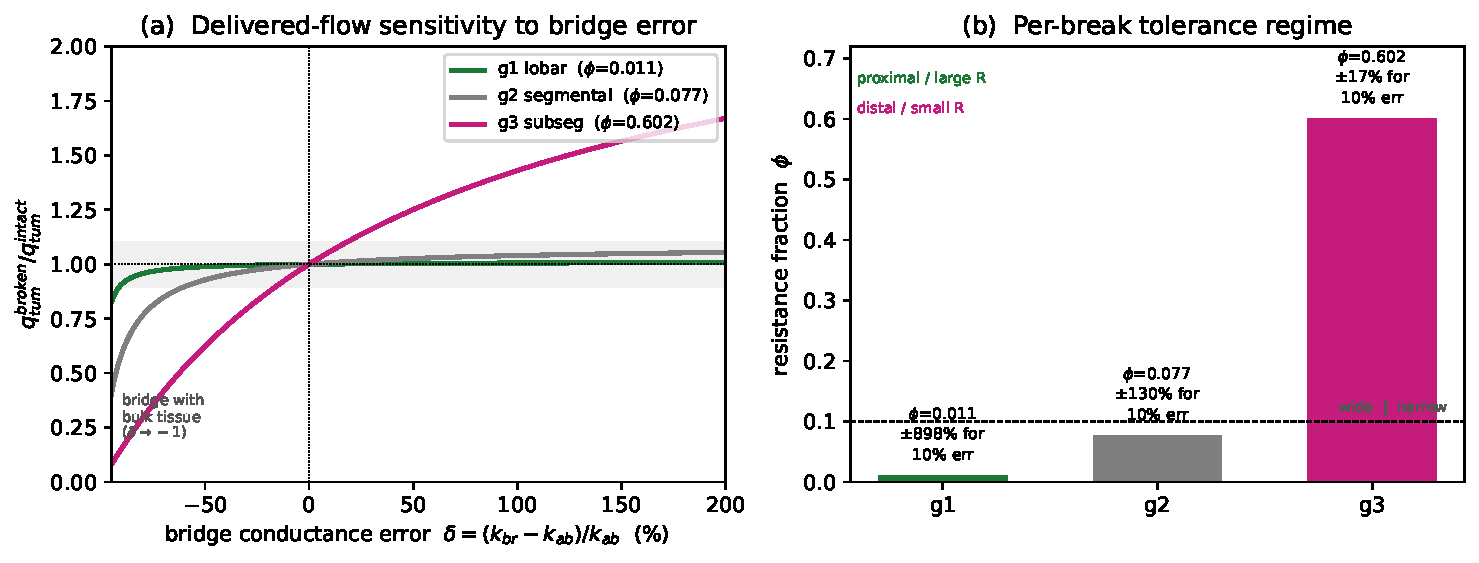
\includegraphics[width=\textwidth]{phi_figure.pdf}
\caption{(a)~Exact delivered-flow ratio versus bridge-conductance error $\delta$ for
a break in each generation; the shaded band marks a $\pm10\%$ flow tolerance. The
proximal curve (g1) is nearly flat---delivered flow is almost independent of how the
break is bridged---while the distal curve (g3) tracks $\delta$ steeply. (b)~The
resistance fraction $\phi$ by generation; annotations give the bridge error
tolerated for a $10\%$ flow error. Breaks with $\phi$ below the dashed line lie in
the wide-tolerance regime and may be bridged crudely; those above require accurate
calibration of $\kbr$ to $k_{ab}$.}
\label{fig:phi}
\end{figure}

\section{Consequence for delivered acid chloride}
\label{sec:dose}

The bolus saturation obeys the 1D advection--reaction transport of Amare et al.,
\begin{equation}
\frac{\partial s_o}{\partial t} + v\,\frac{\partial s_o}{\partial x}
= -\,\Gamma(s_o,\epsilon),
\label{eq:transport}
\end{equation}
advected at the velocity set by the network flow and with a \emph{local} hydrolysis
sink $\Gamma$. Past the outflow node $b$ the advecting field is $\qtum$ and the
reaction term is unchanged by the break. Therefore preservation of $\qtum$ to
tolerance \eqref{eq:tol} implies preservation of the delivered-saturation
(and hence delivered acid-chloride) profile past $b$ to the same first-order
tolerance $\phi\,\delta$. The flow-level equivalence is inherited at the dose level;
the quantity of interest---acid chloride delivered to the tumor---is governed by the
same resistance fraction $\phi$.

\section{Remarks and scope}
\label{sec:scope}

\begin{remark}[Nonlinear embolization]
\label{rem:nonlinear}
Proposition~\ref{prop:port} requires a linear two-port bridge. Once
embolization-driven viscosity feedback engages (as in Onyx/Lipiodol models), $\kbr$
becomes state-dependent and \eqref{eq:exact} holds only in the linearized/local
sense. For the pre-embolization \emph{flow-field} question the two-port reduction and
the equivalence are exact; for the \emph{delivered-dose-with-embolization} question
they furnish the leading-order term plus a state-dependent correction to $\kbr(t)$.
\end{remark}

\begin{remark}[Few generations, exhaustive enumeration]
\label{rem:generations}
In thermoembolization the injection sits within one to three branch generations of
the tumor along a near-straight path, so the set of physically relevant break
configurations---location, width, length across at most three generations---is small
enough to enumerate exhaustively rather than sample, and each is scored by its
$\phi$ from Corollary~\ref{cor:map}.
\end{remark}

\begin{remark}[Reconstruction operator caveat]
\label{rem:mip}
Whether a forward imaging operator that generates realistic breaks is a slab
\emph{mean} or a \emph{maximum-intensity projection} determines which breaks appear:
a mean pulls thin vessels below threshold (partial-volume breaks), whereas a MIP
retains the brightest voxel and suppresses them, leaving only genuinely
intensity-dead gaps. The dominant break mechanism---and thus the operator used to
synthesize ground-truth breaks---should be fixed by comparing, on a large proximal
artery, whether the thick-slab HU matches the mean or the maximum of the thin-slice
HU.
\end{remark}

\end{document}
